
%----------------------------------------------------------------------------------------
%	PREAMBUŁA
%----------------------------------------------------------------------------------------

\documentclass[12pt]{article}
\usepackage[polish]{babel}
\usepackage[T1]{fontenc}
\usepackage{polski}
\usepackage[utf8]{inputenc}
\usepackage{amsmath}
\usepackage{graphicx}
\usepackage{fancyhdr}
\usepackage{float}
\usepackage{graphicx}
\usepackage{hyperref}
\usepackage{verbatim}
\usepackage{listings}

\title{Dokumentacja}
\author{Aleksandra Poręba}

\graphicspath{{static/}} 

\makeatletter
\let\thetitle\@title
\let\theauthor\@author
\let\thedate\@date
\makeatother



 
%----------------------------------------------------------------------------------------
%	STRONA TYTUŁOWA
%----------------------------------------------------------------------------------------
\begin{document}
\begin{center}
\textsc{\normalsize Wydział Fizyki i Informatyki Stosowanej}\\[2.0cm] 

\includegraphics[scale = 1]{logo.png}\\[1cm] 
\textsc{\Large Dokumentacja projektu}\\[0.4cm] 

{ \huge \bfseries \LARGE{Grafowa baza danych POC} }\\[1cm] 

\flushright \Large Aleksandra Poręba \\ nr. indeksu 290514

\vfill 

\center {\today}\\[2cm] 

\pagebreak 

\end{center}

%----------------------------------------------------------------------------------------
%	SPIS TREŚCI
%----------------------------------------------------------------------------------------
\tableofcontents
\pagebreak

%----------------------------------------------------------------------------------------
%	ZAWARTOŚĆ
%----------------------------------------------------------------------------------------

\pagestyle{fancy}
\fancyhf{}

\rhead{\theauthor}
\lhead{\thetitle}
\cfoot{\thepage}

\section{Opis działania aplikacji}
Celem aplikacji było zademonstrowanie użycia grafowej bazy danych.

Aplikacja udostępnia możliwość wyszukiwania najszybszego połączenia pomiędzy przystankami. Użytkownik może dodawanać własne przystanki i relacje między nimi, usuwać je, a także modyfikować.

Na stronie głównej, przestawionej na rysunku \ref{fig:rys1}, znajduje się lista wszystkich dostępnych przystanków w aplikacji.

\begin{figure}[h]
\begin{center}
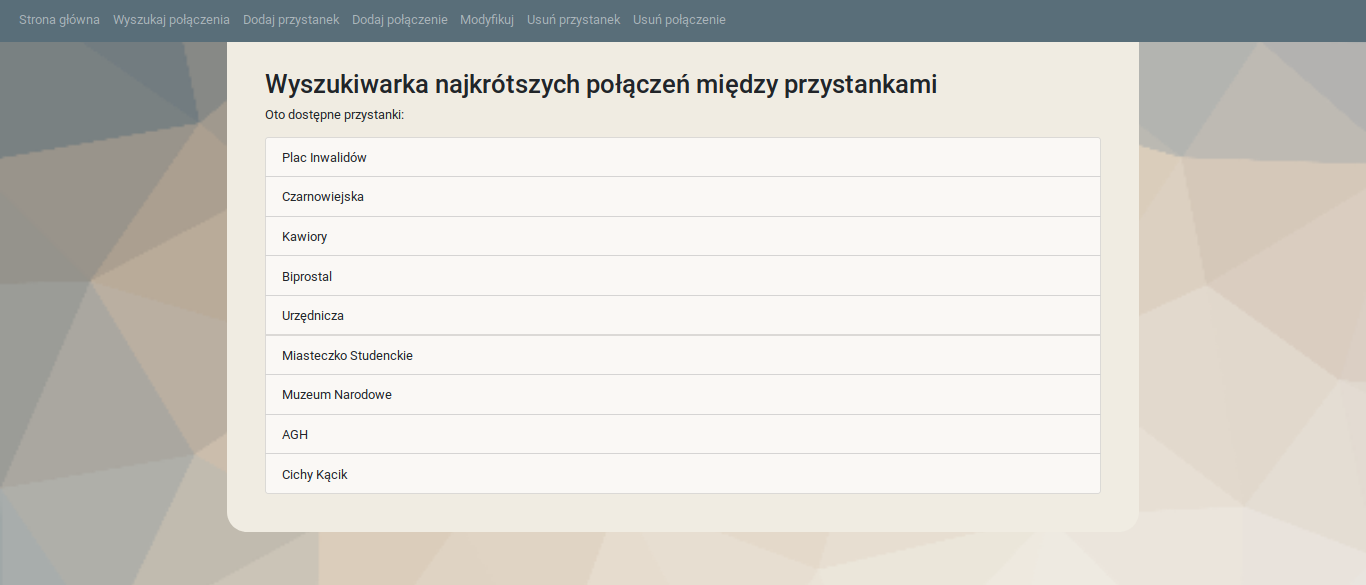
\includegraphics[width=14cm]{strona.png} 
\caption{Strona główna aplikacji} \label{fig:rys1}
\end{center}
\end{figure}

Przemieszczanie po stronie odbywa się za pomocą paska nawigacji.

\subsection{Dodawanie}
W aplikacji możemy dodawać zarówno przystanki (w zakładce ''Dodaj przystanek'') jak i połączenia (w zakładce ''Dodaj połączenie''). Odpowiednie informacje należy podać w formularzu, a następnie potwierdzić przyciskiem ''Dodaj''.

Jeśli użytkownik chce dodać przystanek w formularzu musi podać jego nazwę oraz adres. 

Aby utworzyć nowe połączenie pomiedzy punktami, należy wybrać dwa odpowiednie przystanki z listy, podać numer autobusu (może być też tramwaju), którym możemy odbyć tą trasę oraz szacowany czas przejazdu w minutach.

Aplikacja jest zabezpieczona przed dodaniem nieprawidłowych danych, takich jak puste wartości, za krótka nazwa ulicy, czy wybór dwóch takich samych przystanków.

\subsection{Modyfikacja}
W zakładce ''Modyfikuj'' mamy możliwość zmienienia danych dotyczących przystanku. Po wybraniu nazwy punktu, którego chcemy edytować, zostaje otworzony formularz do zmiany danych z aktualnymi wartościami, pobranymi z bazy.

\subsection{Usuwanie}
Aplikacja udostępnia możliwość usunięcia przystanków razem z wszystkim połączeniami do nich, oraz pojedynczych połączeń. Aby tego dokonać należy wybrać interesujące użytkownika nazwy z listy.

\subsection{Wyszukiwanie}
W zakładce ''Wyszukaj połączenia'' użytkownik może wyszukać najszybszą trasę pomiędzy dwoma przystankami.

\begin{figure}[h]
\begin{center}
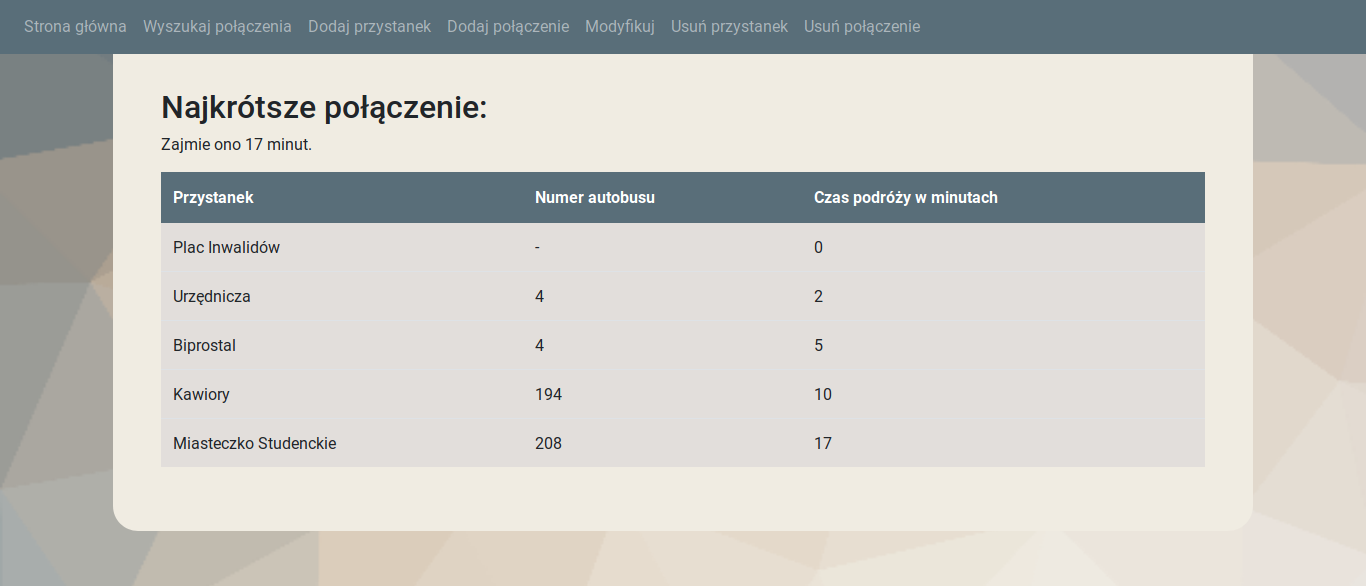
\includegraphics[width=14cm]{wyszukiwanie_duze.png} 
\caption{Przykładowy rezultat wyszukiwania. Aby dojechać z przystanku ''Plac Inwalidów'' do ''Miasteczko Studenckie'' należy pojechać autobusem (tramwajem) numer 4 przez przystanek ''Urzędnicza'' do przystanku ''Biprostal''. Zajmie to 5 minut. Następnie należy przesiąść się na autobus numer 194 i dojechać nim na ''Kawiory''. Ostatnim etapem trasy będzie podróż autobusem 208 do przystanku docelowego. Cała podróż zajmie 17 minut.} \label{fig:rys2}
\end{center}
\end{figure}

 Jako rezultat zostaje wyświetlona tabela z kolejnymi przystankami, numerem autobusu (tramwaju), którym możemy dojechać na dany przystanek, oraz ile czasu podróży już mineło, od jej rozpoczęcia. Przykładowa tabela przedstawiona została na rysunku \ref{fig:rys2}.

\section{Budowa aplikacji}
Projekt składa się z \verb\models.py\, który zawiera model przystanku, komunikujący się z bazą danych, \verb\views.py\ generujący widoki aplikacji oraz \verb\templates\ z szablonami widoków.

\subsection{Modele}
Aplikacja zawiera jeden model danych - model przystanku, który reprezentuje węzeł w bazie. Identyfikowany jest on za pomocą nazwy. Aby wykonać operacje na węzłach wysyłane są zapytania języka Cypher, generowane na podstawie danych przesłanych od widoku z formaularzy. Przykładowe zapytania:
\begin{itemize}
\item dodawanie przystanku 
	\\ \verb\CREATE (p:Przystanek {nazwa:'Kawiory', ulica: 'Nawojki',\
	\\ \verb\	 numer:'1'})\
\item modyfikacja danych przystanku 
	\\ \verb\MATCH (p:Przystanek {nazwa: 'Kawiory'}) SET n.ulica = \
	\\ \verb\'Nawojki', n.numer = '2' RETURN n\
\item usuwanie przystanku 
	\\ \verb\MATCH (p:Przystanek {nazwa: 'Kawiory'}) DETACH DELETE p\
\end{itemize}

Model przystanku operuje też na połączeniach między węzłami, na przykład:
\begin{itemize}
\item dodawanie relacji 
	\\ \verb\ MATCH (p1:Przystanek{nazwa: 'AGH'}), (p2:Przystanek {nazwa:\ 
	\\ \verb\ 		'Kawiory'}) CREATE (p1) - [r:POLACZONY{ numer: '194',\ 
	\\ \verb\ 		czas: 3}]->(p2) RETURN r\ 
\item usuwanie relacji 
	\\ \verb\ MATCH (p1:Przystanek{nazwa: 'AGH'})-[r:POLACZONY]-\ 
	\\ \verb\ 		(p2:Przystanek {nazwa:'Kawiory'}) DELETE r\ 
\item sprawdzanie, czy relacja istnieje 
	\\ \verb\ MATCH (s:Przystanek{nazwa: 'AGH'}), (e:Przystanek {nazwa:\ 
	\\ \verb\ 		'Kawiory'}) RETURN EXISTS ((s)-[:POLACZONY]-(e))\ 
\end{itemize}

Wyszukiwanie najkrótszej ścieżki odbywa się za pomocą zapytania wykorzystującego algorytm Neo4j \verb\algo.shortestPath\:
\\
\\ \verb\MATCH (s:Przystanek {nazwa:'AGH'}), (e:Przystanek {nazwa:'Kawiory'})  \
\\ \verb\	 CALL algo.shortestPath.stream(start, end, 'czas')  \
\\ \verb\	 YIELD nodeId, cost \
\\	\verb\	 RETURN algo.asNode(nodeId).nazwa AS name, cost \

\subsection{Widoki}
W pliku \verb\views.py\ znajdują się funkcje odpowiadające na żądania przekazywane przez obiekt HttpRequest. Widoki generują odpowiednie szablony. Formularze przekazywane są do widoków na pomocą żądania typu POST. Są one najpierw walidowane, a następnie wywoływana jest odpowiednia funkcja modelu. Gdy model zwróci odpowiedź, widok musi odpowiednio na nią zareagować - sprawdzić, czy operacja powiodła się i przeparsować wynik, aby można było go umieścić w szablonie.

\section{Typy danych}
Przystanek w bazie danych jest opisywany poprzez węzeł zawierający trzy atrybuty: nazwę przystanku oraz adres: ulicę i numer. Wszystkie z nich przechowywane są jako łańcuch znaków. Oprócz atrybutów Neo4j dodaje do węzłów indentyfikator.

Przystanki mogą być ze sobą połączone relacją o etykiecie ''POLACZONY''. Zawiera ona dwa artybuty - czas przejazdu podany w minutach oraz numer autobusu (lub tramwaju), którym możemy pokonać daną trasę. Czas przechowywany jest jako liczba całkowita, numer autobusu jako łańcuch znaków (czasem pojawiają się litery przy numerach autobusów, aby określić jego specjalny typ, np. nocny)


\begin{figure}[h]
\begin{center}
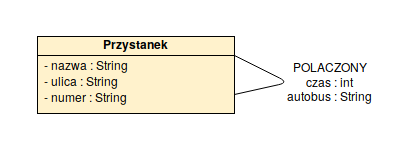
\includegraphics[width=14cm]{uml.png} 
\caption{Model UML} \label{fig:rys3}
\end{center}
\end{figure}


\section{Wykorzystane technologie}
Aplikacja została zrealizowana za pomocą mikroframeworka Flask w języku Python 3. Dostęp do bazy danych jest realizowany przez bibliotekę neo4jrest- client, wysyłającą zapytania do serwera REST bazy Neo4j. Połączenie jest realizowane przez HTTP REST. Baza danych jest dostarczana przez graphenedb, która jest bazą Neo4j w chmurze, hostowana na Heroku.

Do oprawy graficznej strony został użyty framwork Bootstrap4. Szablony widoków uzupełniane są za pomocą Jinja.

Aplikacja znajduje się w środowisku chmurowym Heroku pod adresem:
\url{https://mighty-mountain-55683.herokuapp.com/}.


\section{Bibliografia}
\href{https://devcenter.heroku.com/articles/graphenedb#using-with-python-and-neo4j-rest-client}{Using with Python and Neo4j Rest Client}
\\
\href{https://neo4j.com/docs/cypher-manual/current/}{The Neo4j Cypher Manual v3.5}
\\
\href{https://neo4j-rest-client.readthedocs.io/en/latest/info.html}{neo4j-rest-client’s Documentation}
\\
\href{https://neo4j.com/docs/graph-algorithms/current/}{The Neo4j Graph Algorithms User Guide v3.5}

\end{document}